\documentclass[conference]{IEEEtran}
\IEEEoverridecommandlockouts
% The preceding line is only needed to identify funding in the first footnote. If that is unneeded, please comment it out.
%Template version as of 6/27/2024

\usepackage{cite}
\usepackage{amsmath,amssymb,amsfonts}
\usepackage{algorithmic}
\usepackage{graphicx}
\usepackage{textcomp}
\usepackage{xcolor}
\def\BibTeX{{\rm B\kern-.05em{\sc i\kern-.025em b}\kern-.08em
    T\kern-.1667em\lower.7ex\hbox{E}\kern-.125emX}}

% Added manually:
\usepackage{tikz}
\usetikzlibrary{arrows.meta, positioning, shapes.geometric, fit, backgrounds}
\usepackage{hyperref}
    
\begin{document}

\title{ADLR-Project 18: Efficient Environment Exploration and 3D Reconstruction with Reinforcement Learning and Multiple View Geometry}

% 1\textsuperscript{st} % could be used for 1.
\author{\IEEEauthorblockN{Frank Zillmann}
\IEEEauthorblockA{\textit{Department of Computer Engineering} \\
\textit{Technical University of Munich (TUM)}\\
Munich, Germany \\
frank.zillmann@tum.de}
}

\maketitle

% \begin{abstract}
% This document is a model and instructions for \LaTeX.
% This and the IEEEtran.cls file define the components of your paper [title, text, heads, etc.]. *CRITICAL: Do Not Use Symbols, Special Characters, Footnotes, 
% or Math in Paper Title or Abstract.
% \end{abstract}

% \begin{IEEEkeywords}
% component, formatting, style, styling, insert.
% \end{IEEEkeywords}

\section*{Robosuite Controller Comparison and Recommendations}

\subsection*{MINK vs. non-MINK Whole-Body IK}

\textbf{MINK IK (Minimally-Invasive IK)} attempts to solve the IK problem while 
remaining as close as possible to the previous joint configuration.  
It provides:
\begin{itemize}
    \item Very stable joint motion,
    \item Smooth trajectories without sudden posture jumps,
    \item Robustness for long kinematic chains or redundant robots.
\end{itemize}

\textbf{Non-MINK IK} is a more conventional IK solver:
\begin{itemize}
    \item Slightly simpler numerically,
    \item Often marginally faster per solve (but the difference is typically negligible),
    \item More prone to posture changes, discontinuities, or less intuitive solutions.
\end{itemize}

\textbf{Why not always use MINK?}  
The advantages come with a small cost:
\begin{itemize}
    \item Slightly higher computational overhead (usually a few percent),
    \item Slightly more complex behavior when large configuration changes are needed,
    \item Not needed for simple, non-redundant manipulators.
\end{itemize}

In practice, the IK solver is \emph{never the bottleneck} in a typical robotics pipeline; 
training, simulation physics, or policy inference dominate the runtime by orders of magnitude.
Thus, the speed difference between MINK and non-MINK is usually irrelevant.

\subsection*{Controller Speed Considerations}

\begin{itemize}
    \item \textbf{Whole-Body IK / MINK IK:} Fast (sub-millisecond for standard arms). Far from being a bottleneck.
    \item \textbf{IK\_POSE inside BASIC / WHOLE\_BODY\_COMPOSITE:} Also sub-millisecond. Light-weight differential IK.
    \item \textbf{OSC\_POSE:} Slightly more expensive due to full dynamics (mass matrix, Coriolis, gravity), 
    but still negligible compared to simulation time. Usually well below the physics step time.
\end{itemize}

Thus, \textbf{controller choice is determined by task requirements, not speed}.  
Computation time is effectively never the limiting factor in RL training, simulation, or real-world execution.

\subsection*{Short Summary of Controllers}

\begin{description}
    \item[Whole-Body IK:] Pure geometric IK, fast, joint-position control. No dynamics. 
          Good for simple pose tracking without contact.
    \item[Whole-Body MINK IK:] Same as above but with minimally-invasive optimization. 
          More stable and smoother for redundant robots. Slightly more computation.
    \item[IK\_POSE (BASIC / WHOLE-BODY COMPOSITE):] Differential IK. Joint-velocity control. 
          Good for smooth Cartesian motion, no contact modeling.
    \item[OSC\_POSE:] Full operational-space control with dynamics. Torque-level control. 
          Best for contact-rich or high-precision manipulation.
\end{description}

\subsection*{Recommended Controller for Your Task}

Your task:
\begin{itemize}
    \item Single robot arm,
    \item A camera on the end-effector,
    \item Fully contact-free movement,
    \item Only needs to reach poses and take images.
\end{itemize}

\textbf{Conclusion:}  
For contact-free, pose-based camera movement, the best choices are:
\begin{itemize}
    \item \textbf{Whole-Body IK} (if you want simple point-to-point pose control), or
    \item \textbf{Whole-Body MINK IK} (if you want smoother, more stable, redundancy-aware IK).
\end{itemize}

\textbf{IK\_POSE} is also suitable, but offers no advantage unless you need it 
embedded inside a composite controller.  
\textbf{OSC\_POSE} is unnecessary for non-contact motion and increases controller complexity without benefit.

Thus, use \textbf{Whole-Body IK} for simplest behavior, or \textbf{MINK IK} if your manipulator is redundant and you prefer smooth, minimally-invasive IK trajectories.


\section{RL Problem Structure}
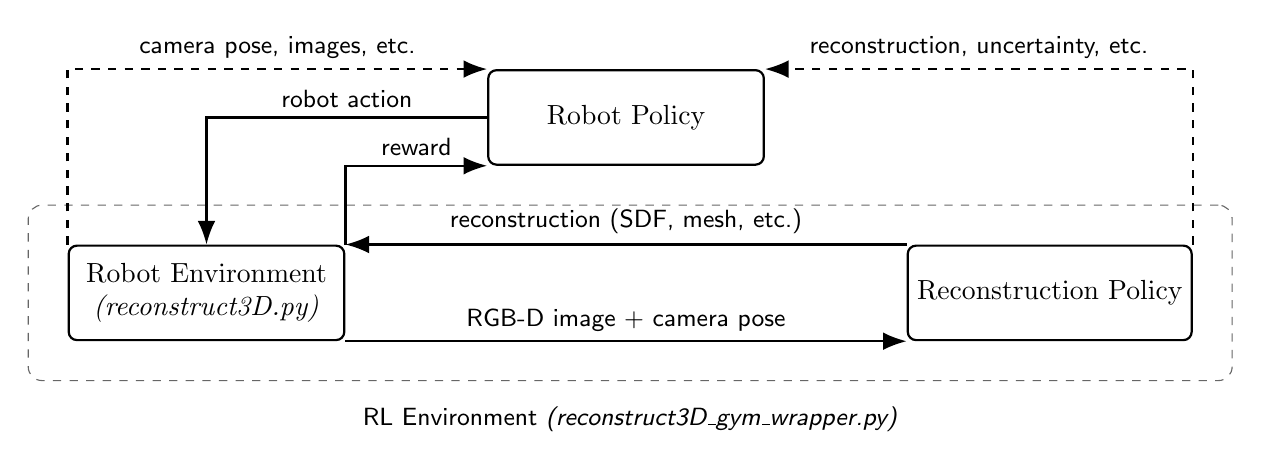
\begin{tikzpicture}[
  box/.style={draw, thick, rounded corners=3pt, minimum width=35mm, minimum height=12mm, align=center},
  arrow/.style={-{Latex[length=3mm]}, thick},
  dashedarrow/.style={-{Latex[length=3mm]}, thick, dashed},
  label/.style={font=\small\sffamily},
]

% --- Node placement (grid-like for zero clutter)
\node[box] (robot)                      {Robot Policy};
\node[box, below left=10mm and 18mm of robot]  (env)   {Robot Environment\\
\textit{(reconstruct3D.py)}};
\node[box, below right=10mm and 18mm of robot] (recon) {Reconstruction Policy};

% --- RL observation region
% \node[
%   draw=blue!60, dashed, rounded corners=5pt,
%   fit=(env)(recon),
%   inner sep=5mm,
% ] (group) {};

\node[
  draw=black!60, dashed, rounded corners=5pt,
  fit=(env)(recon),
  inner sep=5mm,
] (group) {};

\node[
  below=2mm of group,
  label,
  align=center,
  text width=80mm
] {
  RL Environment \textit{(reconstruct3D\_gym\_wrapper.py)}
};

% --- Arrows

\draw[arrow] (robot.west) -| node[label, near start, above]
  {robot action} (env.north);

\draw[arrow] (env.north east) |- node[label, near end, above]
  {reward} (robot.south west);

\draw[arrow] (env.south east) |- node[label, near end, above]
  {RGB-D image + camera pose} (recon.south west);

\draw[arrow] (recon.north west) |- node[label, near end, above]
  {reconstruction (SDF, mesh, etc.)} (env.north east);

% --- Arrows for observations

\draw[dashedarrow] (env.north west) |- node[label, near end, above]
  {camera pose, images, etc.} (robot.north west);

\draw[dashedarrow] (recon.north east) |-
  node[label, near end, above] {reconstruction, uncertainty, etc.} (robot.north east);

\end{tikzpicture}

\bibliographystyle{IEEEtran}
\bibliography{references}

\end{document}